\chapter{Cadre th\'eorique et m\'ethodologique de l'\'etude}
\section*{Introduction}
Les difficult\'es en mati\`ere de qualité des données ne sont pas exclusivement liées aux technologies de l'information, mais il s’agit plutôt d’une problématique qui concerne en grande partie les processus de l’entreprise. Pour mener à bien la présente étude, il est nécessaire d’effectuer un point th\'eorique afin de mieux la situer dans le contexte et de comprendre les r\'eflexions sous-jacentes. Ainsi, ce chapitre fait un résumé de l’existant en matière de cadre d'analyse de la qualit\'e des donn\'ees et amorce la compr\'ehension de l'outil de qualit\'e Apache Griffin. Suite \`a une clarification conceptuelle, nous ferons la lumi\`ere sur les dimensions de qualit\'e de donn\'ees tout en abordant la question des mesures correctives et celle de l'outil \`a choisir.
\section{Clarification conceptuelle}

\subsection{Big Data}
%Pour pouvoir, les utiliser au mieux dans son organisation et son processus décisionnel, il est essentiel de maîtriser les principes et caractéristiques clés du \textit{big data}.
%Le \textit{big data} (donn\'ees massives), fait désormais partie du quotidien de toutes les entreprises. 
Le terme \textit{big data} a été popularisé par John Mashey, informaticien chez Silicon Graphics dans les années 1990 \cite{Cairn_5V}. Ce dernier faisait r\'ef\'erence aux bases de données trop grandes et complexes pour être étudiées avec les méthodes statistiques traditionnelles – et, par extension, à tous les nouveaux outils d’analyse de ces données. En 2001, Douglas Laney a analysé cette nouvelle tendance à travers une liste très simple de trois \textit{« V »}, ensuite élargie à cinq \textit{« V »} \cite{Cairn_5V} \cite{Talend_5V} :
\begin{itemize}[parsep=0cm,itemsep=0cm]
\item le volume : pour d\'esigner la grande quantit\'e de donn\'ees ou d'informations contenues dans ces bases de donn\'ees;
\item la v\'elocit\'e : \'egalement appel\'ee vitesse, correspond à la rapidité à laquelle les donn\'ees sont générées, collect\'ees et circulent pour transmission et analyse;
\item la vari\'et\'e : pour désigner la multiplicité des types de données disponibles, autrement dit les différences de natures, formats et structures \footnote{Donn\'ees structur\'ees, semi-structur\'ees ou non structur\'ees\\};
\item la valeur :  fait r\'ef\'erence \`a la capacit\'e de ces donn\'ees \`a g\'en\'erer du profit; chaque donnée devant apporter une valeur ajoutée à l’entreprise; 
\item la v\'eracit\'e : qui permet de garantir la qualité et la fiabilité des données.
\end{itemize}

%Ces cinq \textit{« V »} permettent donc de d\'ecrire et de caract\'eriser les \textit{big data}. 
Nous nous intéressons ici à cette dernière caract\'eristique. En effet, pour pouvoir tirer de la valeur des donn\'ees, la qualit\'e est la condition pr\'ealable à l'analyse et à l'utilisation du \textit{big data}. D’où la nécessité de prendre des mesures de précaution pour minimiser les biais liés au manque de fiabilité des données. Les méthodes permettant d'améliorer et de garantir la qualité des \textit{big data} sont essentielles pour prendre des décisions commerciales précises, efficaces et fiables. Mais qu'est-ce qu'une donn\'ee de qualit\'e?

%ainsi qu'\`a la garantie de leur valeur

%Dans un contexte o\`u, le volume de données augmente de manière exponentielle, ce sont généralement les entreprises qui commencent à tirer des avantages incroyables de leurs \textit{big data}. Selon les gestionnaires et les économistes, les entreprises qui ne s’intéressent pas sérieusement au \textit{big data} risquent d’être pénalisées et écartées \cite{Lebigdata_5V}. 

%de la valeur contenue dans ces donn\'ees, il leur faut avoir des donn\'ees de qualit\'es, fiables, cr\'edibles et pr\'ecises faisant ainsi r\'eference \`a la v\'eracit\'e.

\subsection{Qualit\'e des donn\'ees}
Définir la qualité des données n’est pas une op\'eration ais\'ee. On est bien souvent tent\'e de définir plut\^ot la non-qualité \cite{pwc_micro_ebg_2011}. Afin de mieux saisir cette notion, nous d\'efinirons d'abord ce qu'on entend par qualit\'e, information et donn\'ee avant de revenir sur la d\'efinition de la qualit\'e des donn\'ees en elle-m\^eme. \`A cet effet, d'apr\`es l'organisation internationale de normalisation (\acrfull{iso}) \cite{Iso8000}, la  qualit\'e pourrait se d\'efinir comme le degré auquel un ensemble de caractéristiques inhérentes à un objet répond aux exigences. On parle \'egalement de conformit\'e aux exigences. Toujours selon l'\acrshort{iso} \cite{Iso8000}, l'exigence se d\'efinit comme un besoin ou une attente énoncée; généralement implicite ou obligatoire. 
Dans \cite{pwc_micro_ebg_2011}, on retiendra que les donn\'ees \emph{« sont des faits et des statistiques qui peuvent être quantifiées, mesurées, comptées, et stockées »} et que l'information quant \`a elle \emph{« est un ensemble de données organisées selon une ontologie\footnote{Une ontologie est l'ensemble structuré des termes et concepts représentant le sens d’un champ d'informations (wikipedia)} qui définit les relations entre certains sujets»}.\\

La qualit\'e des donn\'ees pourrait donc se d\'efinir plus précisément, comme le degré auquel un ensemble de caractéristiques inhérentes aux données répond aux attentes énoncées \cite{Iso8000}. Mais plus loin, Wang et Strong(1996) cit\'es par Cai et Zhu \cite{Cai_Zhu_2015},  d\'efinissent la qualit\'e comme l'aptitude \`a l'emploi et proposent que le jugement de la qualité des données dépende des consommateurs de données. L'objectif est d'avoir \`a disposition des donn\'ees exemptes d'erreurs, d'incohérences, de redondances, de formatage médiocre et d'autres problèmes susceptibles d'empêcher une utilisation aisée \cite{PreciselyDQ}. Ces deux d\'efinitions font ressortir deux aspects tr\`es importants qui se reflètent \'egalement dans la litt\'erature. En effet, tous les auteurs s'accordent sur le fait que la qualit\'e dépend non seulement des caractéristiques propres aux donn\'ees, mais aussi de l'environnement dans lequel ces donn\'ees sont utilis\'ees.
\\

Cette perception met ainsi en exergue le caract\`ere subjectif de cette notion. Aussi peut-on lire \cite{WikiDQ}, que : 
\begin{itemize}[parsep=0cm,itemsep=0cm]
\item pour le consommateur par exemple, des donn\'ees de qualit\'e sont des données : 
\begin{itemize}[parsep=0cm,itemsep=0cm]
\item qui sont aptes à être utilisées ;
\item qui répondent \`a ses attentes ou les dépassent et;
\item  qui satisfont aux exigences de leur utilisation prévue;
\end{itemize}
\item il en est de m\^eme, pour l'entreprise qui de façon sp\'ecifique, inscrit cette d\'efinition dans un cadre op\'erationnel, d\'ecisionnel et commercial;
%\begin{itemize}
%\item  qui sont aptes à être utilisées dans leurs rôles opérationnels, décisionnels et autres prévus ou qui présentent une conformité aux normes qui ont été fixées;
%\item  qui sont adaptées aux utilisations prévues dans le cadre des opérations, de la prise de décision et de la planification et ;
%\item  capable de satisfaire les exigences commerciales, systémiques et techniques déclarées de l'entreprise;
%\end{itemize}
\item par contre, du point de vue des normes, la qualit\'e des donn\'ees est mesur\'ee par :
\begin{itemize}[parsep=0cm,itemsep=0cm]
\item le degré auquel un ensemble de caractéristiques (dimensions de qualité) répond aux exigences ainsi que;
\item l'utilité, la précision et l'exactitude des données pour leur utilisation.
\end{itemize}
\end{itemize}

Cette diversit\'e de point de vue, se justifie par le fait qu'avec l'av\`enement du \textit{big data} contrairement au pass\'e, les utilisateurs de données ne sont pas nécessairement les producteurs de ces données; renforçant de ce fait l'absence d'une d\'efinition unique. Abondant dans le m\^eme sens, sur la d\'efinition de la qualit\'e des donn\'ees, le \acrfull{niss} \cite{NISS_2001} identifie sept(7) principes cl\'es permettant de saisir sa quintessence. Ainsi, ils \'enoncent que les donn\'ees peuvent \^etre vues comme un produit et leur qualit\'e  d\'epend de multiples facteurs et qu'en principe, la qualit\'e peut \^etre  mesurée et améliorée.
\\

Plusieurs dimensions entrent en jeu dans la définition de la qualité. Chacune, décrivant des caractéristiques qui peuvent être mesurées ou évaluées par rapport à des attentes spécifiques \cite{dama}. Le caract\`ere mesurable des dimensions s'av\`ere nécessaire pour leur quantification dans la pratique. On parle alors de m\'etrique. Une métrique de qualit\'e des donn\'ees selon Ehrlinger, Rusz et Wöß \cite{ehrlinger2019survey}, est une fonction qui \`a une dimension de qualité associe une valeur numérique. Une telle métrique peut être calcul\'ee à différents niveaux d'agrégation : au niveau des valeurs, des colonnes ou des attributs, des tuples ou des enregistrements, des tables ou des relations, ainsi qu'au niveau de la base de données. S'adaptent-elles bien au \textit{big data}?
\\

\`A la faveur de cette clarification conceptuelle, on pourrait alors se demander comment mesurer ou \'evaluer la qualit\'e de nos donn\'ees? Quelles sont les dimensions qui existent et quels aspects permettent-elles de capter?



\section{Revue de litt\'erature }
%La qualit\'e des donn\'ees est bien souvent \`a tort r\'eduite \`a une mesure d'exactitude: par exemple, le nom de la ville "Abidjan" mal orthographi\'e en "Abdjan" serait le seul type de probl\`eme rencontr\'e. En effet, on consid\`ere qu'une donn\'ee est de mauvaise qualit\'e si des fautes de frappe sont pr\'esentes ou si des valeurs erron\'ees s'y trouvent. Mais cela ne s'y résume pas. D'autres dimensions plus importantes sont nécessaires pour pleinement la caractériser. Une \'etude de la qualit\'e des donn\'ees ne saurait alors se faire sans avoir clairement identifi\'e des dimensions cibles. Il s'agira ici de faire d'entr\'ee, une revue  des diff\'erents événements qui peuvent entraver la qualit\'e des donn\'ees, pour ensuite d\'eboucher sur quelques dimensions pr\'esentent dans la litt\'erature et enfin les pistes de corrections propos\'ees.

\subsection{D\'efis de la qualit\'e des \textit{big data}}
Le \textit{big data}, loin de ce qu'il pourrait laisser imaginer, n'est \'evidemment pas qu'une simple question de taille. L'extraction et le traitement de donn\'ees de haute qualit\'e,  massives, variables et complexes, deviennent de nos jours une pr\'eoccupation majeure. En effet, l'ère de l'information moderne produit des "tonnes" \footnote{Environ 1,7 m\'egaoctets de données ont \'et\'e g\'en\'er\'ees chaque seconde, par chaque individu tout au long de l'ann\'ee 2020 \cite{dataGen}} de données. Avec l'avènement des téléphones intelligents et de l'internet, des quantités ph\'enom\'enales de données sont cr\'e\'ees. À mesure que le volume et la variété des données augmentent, il devient plus délicat de contrôler chaque entrée afin de s'assurer de leur bonne qualité: les d\'efis \`a relever sont donc \'enormes. Cai et Zhu \cite{Cai_Zhu_2015}, citent quelques d\'efis auxquels le \textit{big data} est confront\'e de nos jours en termes de qualit\'e: 
\begin{itemize}[parsep=0cm,itemsep=0cm]
\item la diversité des sources de données, qui entraîne une abondance de types et de structures complexes, augmente la difficulté de leur intégration;

\item le volume énorme des données, rend difficile l'appr\'eciation de la qualit\'e dans un d\'elai raisonnable;

\item la prise en compte du temps réel dans l'\'evaluation de la qualit\'e; 

\item l'inexistence de normes unifiées et approuvées de qualité des données et; 

\item les r\'eflexions sur la qualité des \textit{big data} sont relativement r\'ecentes.
\end{itemize}

Ces d\'efis demeurent d'actualit\'e d'autant plus qu'aucune entreprise ne saurait aspirer \`a une r\'eelle expansion sans int\'egrer le \textit{big data} et une v\'eritable strat\'egie de gouvernance des donn\'ees. 
%Voil\`a donc, les d\'efis qu'une entreprise \`a la recherche d'un cadre m\'ethodologique d'analyse de la qualit\'e de ses \textit{big data} doit relever. 

\subsection{Sources de non-qualit\'e}
Les problèmes de qualité de données surviennent lorsque les exigences qualité ne sont pas satisfaites. Mais surtout, ces problèmes sont d\^us à plusieurs facteurs ou processus. En effet, comme l'indique Taleb, Serhani et Dssouli \cite{BigDataQlt}, Ben Salem \cite{bensalem}, pwc \cite{pwc_micro_ebg_2011} et \cite{TalanConsulting}, les sources de non-qualit\'e couramment rencontr\'ees sont:
\begin{itemize}[parsep=0cm,itemsep=0cm]
\item l'entr\'ee manuelle des donn\'ees ;

\item la dégradation de la donnée dans les chaînes et processus de traitement (troncatures, caractères mal interprétés, erreurs de conversions, absence de contrôles sur le format, passage d'un syst\`eme d'encodage \`a un autre,...);

\item la corruption volontaire ou intentionnelle des donn\'ees \`a des fins malhonnêtes;

\item l'existence de données non actualisées qui deviennent une source d’inexactitude avec le temps;

%\item des défauts de conception qui en laissant subsister une ambiguïté sémantique peuvent amener à des erreurs de valorisation et également d'interprétation de la donnée par la suite;

\item l'absence de contraintes d'intégrités et de procédures pour maintenir la cohérence des donn\'ees;

\item le manque de rigueur dans la définition des attributs;

\item l'int\'egration de donn\'ees provenant de sources externes et faisant l'objet de contradictions ou d'incoh\'erences avec celles locales.

\end{itemize}
%\vspace {0.5cm}

Combin\'ees avec les caract\'eristiques majeures du \textit{big data}, la complexité de l’organisation d’une entreprise et la multiplicité des chaînes de traitement augmentent le risque de tous ces facteurs. Dans ces conditions, plus l’anomalie ou la non-qualité est détectée tôt, suivie et corrigée à la source, plus fiable sera l’ensemble du patrimoine global de données. D'o\`u la nécessité d'un outil d'audit de la qualit\'e des donn\'ees. Mais avant de penser \`a l'outil, il serait judicieux de se pencher sur les aspects de la qualit\'e qu'on souhaite aborder. C'est pour cela qu'il est important d'analyser les dimensions de qualité existantes, largement utilisées pour évaluer la qualité des données, afin de déterminer dans quelles mesures elles sont applicables au \textit{big data}. 


%outdated values
%incomplete values
%conflicting values
%wrong values
%noise in the data extraction.


%(parler de data gouvernance)
%L’entreprise utilise différents types de données qui peuvent être saisies ou collectées de diverses manières et qui sont destinées à des usages différents :

\subsection{\'Evaluation de la qualit\'e des donn\'ees}

Pour garantir des donn\'ees d'une certaine qualit\'e aux utilisateurs, chaque organisation se doit de d\'efinir les dimensions qu'elle utilisera dans son processus. Ben Salem \cite{bensalem}, pr\'ecise que chaque organisme doit créer ses propres définitions opérationnelles en fonction de ses objectifs et priorités, de sorte \`a déterminer des indicateurs pour chacune des dimensions choisies, et vérifier par des mesures régulières leur évolution dans le temps. 
Pour les données structurées, la littérature  propose diff\'erentes dimensions.

%Les données doivent avoir la qualité nécessaire pour supporter le type d’utilisation pr\'evue. 
%La clarification conceptuelle sur la qualité des données a permis de comprendre qu'il s'agit d'un concept aux multiples facettes, et différentes dimensions concourent à la définir.

\subsubsection{\textbf{Dimensions de la qualit\'e des donn\'ees}}  
Bien que relativement r\'ecents, les travaux sur les dimensions de la qualit\'e des donn\'ees ont mis en exergue un ensemble de dimensions. Plusieurs auteurs se sont pr\^et\'es \`a cet exercice de revue des diff\'erentes dimensions utilis\'ees pour attester de la qualit\'e d'un ensemble de donn\'ees. Notre \'etude porte principalement sur l'utilisation d'Apache Griffin, comme outil d'audit de la qualit\'e des donn\'ees. Ce dernier, s'inspire de la définition de la \acrfull{dama} \cite{dama}, qui identifie six principales dimensions pour l'\'evaluation de la qualit\'e des donn\'ees \cite{dama}, \cite{ehrlinger2019survey} :

\begin{enumerate}
\item \textbf{l'exhaustivité ou la complétude (\textit{completeness})} : qui mesure l'absence de valeurs manquantes (chaînes de caractères nulles ou vides, donn\'ees  num\'eriques manquantes). Il est à noter que le nombre de valeurs manquantes peut être calculé de différentes manières, soit en ne prenant en compte que les vraies valeurs manquantes (c'est-\`a-dire \textit{null}), soit les valeurs par défaut ou une entrée textuelle mentionnant "\acrshort{nan}" (c'est-à-dire, \acrlong{nan});

\item \textbf{l'unicité (\textit{uniqueness})} : cette dimension permet l'analyse des valeurs uniques. L'unicité est l'inverse d'une évaluation des doublons. %Ces deux aspects repr\'esentent les faces d'une m\^eme pi\`ece;

\item \textbf{l'actualité (\textit{timeliness})} :  décrit le degré de fra\^icheur des données pour la tâche à accomplir et est étroitement liée aux notions de fréquence de mise à jour des données  et de volatilité (vitesse à laquelle les données deviennent non pertinentes). Une autre définition indique que l'actualité peut être interprétée comme la probabilité qu'un attribut soit toujours à jour \cite{ehrlinger2019survey}. Elle se mesure en détectant le taux de valeurs obsolètes dans la base de données par rapport à une date prédéfinie ou en analysant la latence entre les diff\'erentes entr\'ees. Cette dimension sied plus aux donn\'ees en \textit{streaming};

\item \textbf{la validité (\textit{validity})} : une donnée est jug\'ee valide si elle est conforme aux exigences de sa définition : format (email, date), type (num\'erique, r\'eel), plage (intervalle de variation). Il s'agit d'une comparaison entre les données et les métadonnées ou la documentation ; 


\item \textbf{l'exactitude (\textit{accuracy})} : cette dimension \'evalue la mesure dans laquelle un syst\`eme d'information décrit correctement ou se rapproche du monde réel qu'il est censé modéliser. Elle se mesure en d\'etectant le taux de valeurs correctes ou incorrectes dans la base de données au regard d'une source de donn\'ees d\'efinie comme r\'ef\'erence : "source.colonne": "address", "reference.colonne": "address";

\item \textbf{la cohérence (\textit{consistency})} : selon Batini et Scannapieco cit\'es par Ehrlinger, Rusz et Wöß \cite{ehrlinger2019survey} , la cohérence capture la violation des règles sémantiques définies sur les données, où les éléments peuvent être des tuples de tables relationnelles ou des enregistrements dans un fichier. Les contraintes d'intégrité de la théorie relationnelle sont un exemple de telles règles. La coh\'erence se mesure donc par rapport \`a l'ensemble des contraintes en d\'etectant les donn\'ees qui ne les satisfont pas. 

\begin{figure}[!h]
  \caption{Dimensions de la qualit\'e des donn\'ees selon la DAMA UK}  \label{fig:dama_uk}
  \begin{center}
    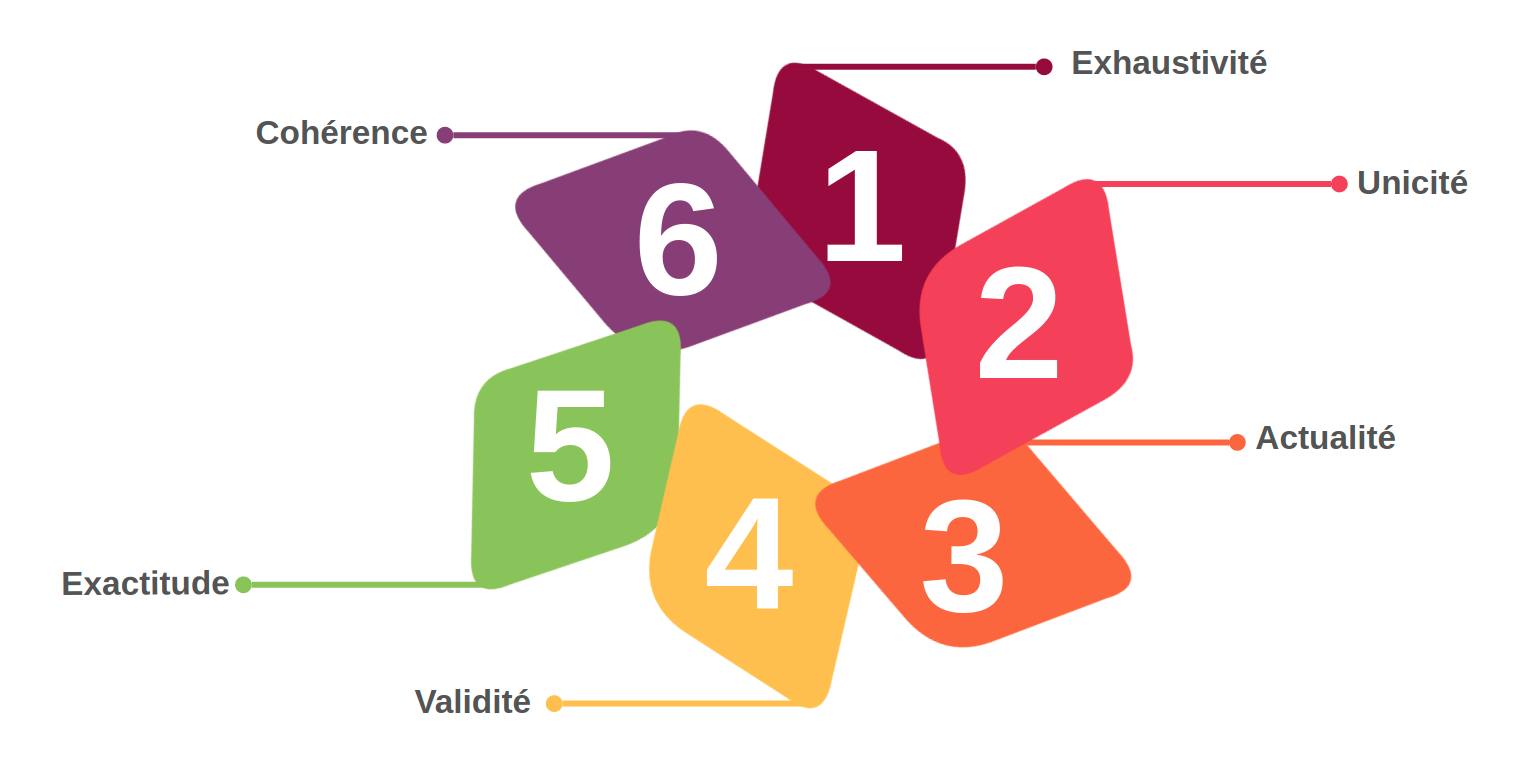
\includegraphics[scale=0.33]{Static/Dim3.png} 
  \end{center}
\end{figure}

\end{enumerate}
\vspace {0.5cm}

Dans une tentative de synth\`ese, Berti-Equille \cite{BertiEquille2004} fait remarquer en 2004 que quel que soit le domaine d’application, les mesures de qualité de données les plus fréquemment mentionnées, sont l'exactitude, la complétude, l’actualité et la cohérence. Mais nous retiendrons pour cette \'etude les six dimensions susmentionn\'ees.

\subsubsection{\textbf{Dimensions de la qualit\'e des donn\'ees \`a l'\`ere du \textit{big data}}}

De nos jours, les \textit{big data} imposent de nouveaux défis liés à leurs principales caractéristiques. En particulier, afin d'aborder les questions de volume et de vélocité, il est nécessaire de repenser les méthodes d'évaluation pour exploiter les scénarios de calcul parallèle. Mais aussi, il revient de se demander si les dimensions de qualit\'e existantes sont toujours d'actualit\'e ou n\'ecessitent des ajustements. Ainsi, pour \'evaluer la qualit\'e des \textit{big data}, Cai et Zhu \cite{Cai_Zhu_2015} proposent une hi\'erarchie de dimensions et de sous-dimensions: 
\begin{itemize}

\item[>] la \textbf{disponibilit\'e} de la donn\'ee caract\'eris\'ee par:
\begin{itemize}[parsep=0cm,itemsep=0cm]
\item l'accessibilit\'e:  existe-t-il des facilit\'es d'acc\`es aux donn\'ees?; 
\item l'actualit\'e: la donn\'ee est-elle r\'eguli\`erement mise \`a jour?;
\item l'autorisation: a-t-on le droit d'utiliser ces donn\'ees? a-t-on les acc\`es n\'ecessaires ?;
\end{itemize}
%\vspace {0.5cm}

\item[>] l'\textbf{utilisabilit\'e}  de la donn\'ee caract\'eris\'ee par:
\begin{itemize}[parsep=0cm,itemsep=0cm]
\item l'existence d'une documentation;
\item la cr\'edibilit\'e : qui concerne la fiabilit\'e de la source de donn\'ees, la normalisation des donn\'ees et le moment o\`u les donn\'ees sont produites;
\item l'existence de m\'eta-donn\'ees;
\end{itemize}
%\vspace {0.5cm}

\item[>] la \textbf{fiabilit\'e} de la donn\'ee caract\'eris\'ee par quatre des six dimensions identifiées par la \acrshort{dama} \cite{dama}:
\begin{itemize}[parsep=0cm,itemsep=0cm]
\item l'exactitude;
\item l'int\'egrit\'e ou validit\'e \cite{dama} ;
\item la coh\'erence;
\item la compl\'etude;
\item l'auditabilit\'e : l'auditabilité signifie que l'exactitude et l'intégrité des données  peuvent être évaluer équitablement dans des limites de temps et de main-d'œuvre rationnelles ;
\end{itemize}
%\vspace {0.5cm}

\item[>] la \textbf{pertinence} de la donn\'ee caract\'eris\'ee par:
\begin{itemize}
\item l'aptitude de la donn\'ee \`a satisfaire son utilisateur;
\end{itemize}
%\vspace {0.5cm}

\item[>] la \textbf{qualit\'e de la pr\'esentation} caract\'eris\'ee par:
\begin{itemize}[parsep=0cm,itemsep=0cm]
\item la lisibilit\'e : est-ce que la donn\'ee est bien d\'efinie suivant une terminologie connue et courante ?;
\item la structuration : la structure fait référence \`a la difficulté à transformer les données semi-structurées ou non structurées en données structurées.
\end{itemize}
\newpage
\begin{figure}[!h]
  \caption{Hiérarchisation des dimensions selon Cai et Zhu}  \label{fig:cai_shu}
  \begin{center}
    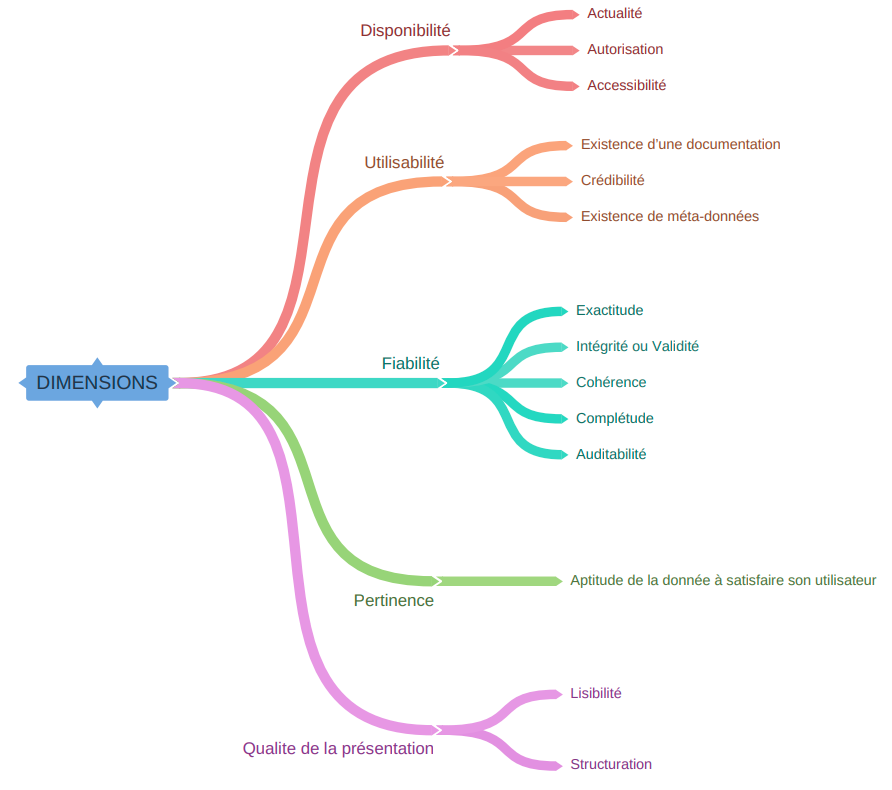
\includegraphics[scale=0.6]{Main/Static/Dimensions_Screen.png} 
  \end{center}
\end{figure}

\end{itemize}  
%\vspace{0.5cm}

Plusieurs autres auteurs ont \'egalement propos\'e des cadres m\'ethodologiques d'analyse de la qualit\'e des \textit{big data}. Ramasamy et Chowdhury \cite{articleRamasamyChowdhury2020} en font une pr\'esentation succincte r\'esum\'e. En plus de l'accessibilit\'e \cite{Cai_Zhu_2015}, la lisibilit\'e \cite{Cai_Zhu_2015}, la cr\'edibilit\'e et la confiance \cite{articleRamasamyChowdhury2020} (la cr\'edibilit\'e \cite{Cai_Zhu_2015}), la coh\'esion \cite{articleRamasamyChowdhury2020} (la coh\'erence \cite{dama}, \cite{Cai_Zhu_2015}) ainsi que la confidentialit\'e \cite{articleRamasamyChowdhury2020} (l'autorisation \cite{Cai_Zhu_2015}), ils font ressortir quatre autres dimensions jug\'ees importantes : 

\begin{itemize}[parsep=0cm,itemsep=0cm]
\item le p\'edigr\'ee ou la lignée : cette dimension permet de connaître la source des donn\'ees afin d'y corriger les éventuelles incoh\'erences ;
\item la capacit\'e d'analyse en temps r\'eel;
\item la redondance :  elle fait r\'ef\'erence \`a la capacit\'e \`a repr\'esenter le monde r\'eel sans r\'ep\'etition des informations ;
\item le volume : cette dimension permet d'analyser le volume des donn\'ees extraites.

\end{itemize}
\vspace {0.5cm}

Au regard des dimensions \'enum\'er\'ees, on constate que plusieurs d'entre elles int\`egrent le fait que les \textit{big data} ne sont pas forc\'ement produites en entreprise, mais pour la plupart proviennent de sources externes et que cela a un impact sur la qualit\'e. Ainsi, on peut distinguer des dimensions qui sont quantifiables et d'autres ayant un aspect plus qualitatif. On retiendra néanmoins que les dimensions retenues pour les donn\'ees structur\'ees demeurent quand m\^eme applicables dans le contexte des \textit{big data}.
%Mettre en place des indicateurs de performance pour piloter la qualité des données est un acte fondateur témoignant du sérieux de l’entreprise dans sa démarche. C’est  une condition du succès, comme nous le rappelle Thierry Savit :
%Before attempting to use data quality dimensions, an organisation needs to agree the quality rules against which the data needs to be assessed against. 
%nous allons donc dans un premier temps pr\'esenter les dimensions qui ont inspir\'e celles impl\'ement\'ees.

\subsubsection{\textbf{Outils d'\'evaluation de la qualit\'e des donn\'ees}}
L'\'evaluation de la qualit\'e suivant les diff\'erentes dimensions retenues par l'entreprise, ne peut se faire efficacement de façon manuelle. Elle nécessite l'utilisation d'un outil ou d'une plateforme sp\'ecialement d\'edi\'e \`a cette t\^ache. Trois (3) options s'offrent aux entreprises \cite{linkedinDeepakRout}:
\begin{description}[parsep=0cm,itemsep=0cm]
\item[un outil fait maison:] cette approche requiert un énorme investissement en terme de travail afin de mettre en place un outil facilement adapt\'e aux diff\'erentes sources de donn\'ees; mais offre tous les avantages li\'es \`a la disposition d'un outil personnalis\'e et facilement maintenable. Elle convient aux grandes organisations disposant d'une grosse \'equipe de d\'eveloppement rompue \`a cette t\^ache;
\item[un outil open source: ] il s'agit de l'approche la plus courante. La gratuité, la connectivité avec la majorit\'e des environnements de données modernes ainsi que la disponibilité des fonctionnalités nécessaires en font un choix de premier ordre. Les plus populaires sont: Apache Griffin, Deequ, Great Expectations, MobyDQ, Data Validator, Bigdata Profiler.
\item[une solution commerciale: ] elles sont pour la plupart d\'evelopp\'ees par des fournisseurs de solutions \acrfull{etl}. Et conviennent mieux aux organisations ayant déjà souscrit \`a un produit en provenance de la m\^eme entreprise. Elles offrent l'avantage d'avoir un support technique et une int\'egration transparente avec l'\acrshort{etl} en d\'epit du co\^ut des licences. Quelques exemples de ces produits sont les offres de Talend (Talend Data Quality) et Informatica (Talend Data Quality). 
\end{description}
%\begin{landscape}

Nous nous intéressons particuli\`erement aux solutions open source, plus précisément \`a Apache Griffin. Nous pr\'esentons un rapide comparatif des outils les plus en vue du march\'e.

%\begin{footnotesize}

\begin{table}[H]
\caption{Comparaison de Apache Griffin - Great Expectations - Deequ}
\footnotesize
%\begin{adjustwidth}{-3em}{-1em}%{-4em}{-1em}small
\vspace{0.5cm}
\begin{tabular}{ll|cl|cl|cl}%>{\justify}p{3cm}>{\justify}p{3cm}>{\justify}p{3cm}
\toprule 
                          && \textbf{Apache Griffin}     && \textbf{Great Expectations}     && \textbf{Deequ}               \\%& mobyDQ & data-validator & bigdata-profiler  \\
\midrule
%\rowcolor{lightgray}

                          && Pr\'ed\'efinies     && Pr\'ed\'efinies         && Pr\'ed\'efinies        \\%& Pr\'ed\'efinie (faible vari\'et\'e) & Pr\'ed\'efinie & Pr\'ed\'efinie \\
\textbf{R\`egles}                  && et personnalisables  && (Riches et vari\'ees)  && (Riches et vari\'ees)         \\%& Pr\'ed\'efinie (faible vari\'et\'e) & Pr\'ed\'efinie & Pr\'ed\'efinie \\
\textbf{de qualit\'e}              &&  en utilisant      &&  et personnalisables     && Comp\'etences en          \\%& Pr\'ed\'efinie (faible vari\'et\'e) & Pr\'ed\'efinie & Pr\'ed\'efinie \\
                          &&  du SQL            &&    (Python)            && Scala \\%& Pr\'ed\'efinie (faible vari\'et\'e) & Pr\'ed\'efinie & Pr\'ed\'efinie \\
\hline 
\textbf{Profiling}                 && Manuel             && Automatique            && Automatique               \\%& - & - & -\\ 

\hline
\textbf{Suggestions}               && Non                && Oui                    && Oui                         \\%& Non & Non & Non\\ 
\textbf{de r\`egles }              &&                    &&                        &&                              \\%& Non & Non & Non\\ 

\hline
\textbf{Stockage des}              && Elasticsearch,HDFS && JSON                   && Configurable                  \\%& PostgreSQL & - & DogStatsD\\ 
\textbf{m\'etriques}               && Personnalisable    &&                        && Spark DataFrame                               \\%& PostgreSQL & - & DogStatsD\\ 

\hline
\textbf{D\'etection d'anomalies}    && Pas encore         && Non                    && Oui                              \\%& Non & Non & Non\\ 

\hline 
\textbf{Documentation automa-}             &&                    &&                        &&                                   \\%& IU & - & -\\ 
\textbf{tique des m\'etriques/}          && IU                 && Documentation          && -                                  \\
\textbf{Interface Utilisateur(IU)}     &&                    &&                        &&                                     \\

\hline 
\textbf{}                    && JDBC,Avro,Hive        && SGBDR,                 && Toutes sources                       \\%&  & Hive, OrcFile,Parquets & CSV,JSON,Parquet\\ 
 \textbf{Source de donn\'ees}                       && Hadoop,Fichiers plat,    &&S3                      && support\'ees                         \\%&  & Hive, OrcFile,Parquets & CSV,JSON,Parquet\\ 
\textbf{}                 && Personnalisable       &&Fichiers plat              && par Spark                            \\%&  & Hive, OrcFile,Parquets & CSV,JSON,Parquet\\ 

\hline 
\textbf{Langage}                   && Scala              && Python                 && Scala                       \\%& Python & Scala & Scala\\ 
                          &&\& SQL              &&                        && \& Interface Python          \\%& Python & Scala & Scala\\ 

\hline 
\textbf{Support technique/}        && Apache             && Professionnel          && AWS                           \\%& Ubisoft & - & - \\ 
\textbf{communaut\'e }             &&                    &&  et communaut\'e       &&                                \\%& Ubisoft & - & - \\ 

\hline 
\textbf{Documentation}             && D\'etaill\'ee      && D\'etaill\'ee          && D\'etaill\'ee                   \\%& D\'etaill\'ee  & Minimaliste  & Pauvre \\

\hline 
\textbf{Volume de donn\'ees}       && Petaoctet         && Gigaoctet              &&  -                             \\%& D\'etaill\'ee  & Minimaliste  & Pauvre \\ 

\hline 
\textbf{API}                       && Oui                && Non                    && Non                                \\%& D\'etaill\'ee  & Minimaliste  & Pauvre \\ 

\hline 
\textbf{Environnement}             && Hadoop             && Pandas,SQL,BigQuery    &&                                  \\%& D\'etaill\'ee  & Minimaliste  & Pauvre \\ 
\textbf{d'ex\'ecution}             && Spark              && Redshift, Spark, mais  && Spark                             \\%& D\'etaill\'ee  & Minimaliste  & Pauvre \\ 
                          && Hive               && optimis\'e pour Python &&                                   \\%& D\'etaill\'ee  & Minimaliste  & Pauvre \\ 

\hline 
\textbf{Alerte}                    && Email              && Email/Slack 			&&                                    \\%& D\'etaill\'ee  & Minimaliste  & Pauvre \\ 

\hline 
\textbf{Modes}                     && Batch et Streaming && Batch                  && Batch                               \\%& D\'etaill\'ee  & Minimaliste  & Pauvre \\ 

\hline 
\textbf{Ex\'ecution}               && Oui                && Apache                 &&                                      \\%& D\'etaill\'ee  & Minimaliste  & Pauvre \\ 
\textbf{programm\'ee}              && crontab            && Airflow                &&                                      \\%& D\'etaill\'ee  & Minimaliste  & Pauvre \\ 

\bottomrule
\end{tabular}
%\end{adjustwidth}

\end{table}
%\end{footnotesize}
%\end{landscape}

%\newpage

\begin{table}[H]
\caption{Comparaison de mobyDQ - data-validator - bigdata-profiler}

%\begin{adjustwidth}{-1em}{-2em}%{-1em}{-2em}small
\vspace{0.5cm}
\footnotesize
\setlongtables
\begin{longtable}{ll|cl|cl|cl}%>{\justify}p{3cm}>{\justify}p{3cm}>{\justify}p{3cm}
\toprule 

                                         &&  \textbf{mobyDQ}               && \textbf{data-validator}   && \textbf{bigdata-profiler}                     \\
\midrule
\endhead
                                         && 	Pr\'ed\'efinies	           &&                           && N\'ecessite des                      \\%
\textbf{R\`egles}                        &&    mais faible                 && Pr\'ed\'efinies           && comp\'etences en                     \\
\textbf{de qualit\'e}                    &&   vari\'et\'e                  && (Riches et vari\'ees)     && programmation                        \\
                                         &&  de r\`egles                   &&                           && scala                                \\
\hline 

\textbf{Profiling}                       && Non                            && Non                       && Non                                  \\%& - & - & -\\ 
\hline

\textbf{Suggestions}                     && Non                            && Non                       && Non                                  \\%& Non & Non & Non\\ 
\textbf{de r\`egles}                     &&                                &&                           &&                                      \\%& Non & Non & Non\\ 
\hline

\textbf{Stockage des}                    &&PostgreSQL                      && JSON                      && DogStatsD                            \\%& PostgreSQL & - & DogStatsD\\ 
\textbf{m\'etriques}                     &&                                &&                           &&                                      \\%& PostgreSQL & - & DogStatsD\\ 
\hline

\textbf{D\'etection d'anomalies }         && Non                            && Non                       && Oui                                  \\%& Non & Non & Non\\ 
\hline 

\textbf{Documentation automa-}                   &&                                &&                           &&                                      \\%& IU & - & -\\ 
\textbf{tique des m\'etriques}                 && IU                             && Aucun                     && Aucun                                \\
\textbf{Interface Utilisateur(IU)}       &&                                &&                           &&                                      \\
\hline 

                                         && SGBDR,Snowflake                && OrcFile,                  && CSV,                       \\%&  & Hive, OrcFile,Parquets & CSV,JSON,Parquet\\ 
\textbf{Source de donn\'ees}             && Impala,Teradata                && Parquet,                  && Parquet,                         \\%&  & Hive, OrcFile,Parquets & CSV,JSON,Parquet\\ 
                                         && Hive                           && Hive                      && JSON                            \\%&  & Hive, OrcFile,Parquets & CSV,JSON,Parquet\\ 
\hline 

\textbf{Langage}  						 && Python                         && Scala                     && Scala                                \\%& Python & Scala & Scala\\ 
\hline 

\textbf{Support technique/}              && Ubisoft                        &&                           &&                                      \\%& Ubisoft & - & - \\ 
\textbf{communaut\'e}                    &&                                &&                           &&                                      \\%& Ubisoft & - & - \\ 
\hline 

\textbf{Documentation}                   && D\'etaill\'ee                  && Minimaliste               && Pauvre                               \\%& D\'etaill\'ee  & Minimaliste  & Pauvre \\
\hline 
 
\textbf{Volume de donn\'ees}             && -                              && -                         && -                                    \\%& D\'etaill\'ee  & Minimaliste  & Pauvre \\ 
\hline 

\textbf{API}                             && Oui                            && Non                       && Non                                  \\%& D\'etaill\'ee  & Minimaliste  & Pauvre \\ 
\hline 

\textbf{Environnement}                   &&  Nginx                         &&                           &&                                      \\%& D\'etaill\'ee  & Minimaliste  & Pauvre \\ 
\textbf{d'ex\'ecution}                   &&  Python                        && Spark                     && Spark                                \\%& D\'etaill\'ee  & Minimaliste  & Pauvre \\ 
                                         &&  GraphQL                       &&                           &&                                      \\%& D\'etaill\'ee  & Minimaliste  & Pauvre \\ 
\hline 

\textbf{Alerte}                          && Email                          && Email                     && Non                                  \\%& D\'etaill\'ee  & Minimaliste  & Pauvre \\ 
\hline 

\textbf{Modes}                           && Batch                          && Batch                     && Batch                                \\%& D\'etaill\'ee  & Minimaliste  & Pauvre \\ 
\hline 

\textbf{Ex\'ecution}                     && Non                            && Oui                       && Possible                                   \\%& D\'etaill\'ee  & Minimaliste  & Pauvre \\ 
\textbf{programm\'ee}                    &&                                && crontab                   &&                                      \\%& D\'etaill\'ee  & Minimaliste  & Pauvre \\ 
\bottomrule
\end{longtable}
%\end{adjustwidth}

\end{table}
%\newpage
\subsection{Anomalies et Mesures correctives}
\subsubsection{\textbf{Diff\'erents types d'anomalies}}

Les données jouent un r\^ole crucial pour prendre les bonnes décisions à propos de la direction future de l’entreprise, et comme le dit l'adage \textit{«\`a données inexactes, résultats erronés»}. Les anomalies dans les données sont très variées et sont causées par plusieurs facteurs. Dans \cite{IFP}, on retrouve cinq (5) des probl\`emes les plus courants en mati\`ere de qualit\'e des donn\'ees. De son c\^ot\'e, Ben Salem \cite{bensalem}  met en évidence huit (8) classes d'anomalies dans les donn\'ees regroupant aussi bien les r\'esultats de \cite{IFP} que ceux de Todoran \cite{todoran}. Essentiellement nous avons: 

\begin{itemize}[parsep=0cm,itemsep=0cm]
\item \textbf{l'incohérence des formats, la codification des donn\'ees, la multiplicit\'e des langues et des unit\'es de mesures} : on d\'esigne ici l'existence de formatages diff\'erents pour la m\^eme donn\'ee; par exemple la date aux formats JJ/MM/AAAA et MM/JJ/AAAA, le format des donn\'ees de type num\'erique doit \^etre clairement pr\'ecis\'e. Comme pour le formatage, les différences de langue, d'alphabet ou d'unités de mesure peuvent g\'en\'erer des erreurs (caractères sp\'eciaux;  fahrenheit ou celsius);

\item \textbf{les valeurs erronées, les valeurs aberrantes (commun\'ement appel\'ees \textit{outliers})}: ce type d'anomalie est le plus souvent rencontré. Un \textit{outlier} est une valeur qui est anormale par rapport au comportement des autres valeurs. Une valeur erronée d\'esigne en revanche une valeur diff\'erente de celles attendues. Elles sont parfois difficiles \`a d\'etecter surtout si le formatage reste acceptable;

\item \textbf{les donn\'ees incompl\`etes ou valeurs manquantes}: elles se manifestent par l'absence partielle ou totale d'informations pertinentes (ou non), laissant place \`a des champs partiellement remplis ou laiss\'es blancs. Todoran \cite{todoran}, fait remarquer que les données incomplètes repr\'esentent un type d'imperfection qui affecte surtout les bases de données volumineuses. Elles ne sont pas toutes de même nature. On distingue selon la classification faite par Little et Rubin (1987) cit\'e par Glasson-Cicognani et Berchtold \cite{glassoncicognani}, les :
\begin{itemize}[parsep=0cm,itemsep=0cm]
\item \acrfull{mcar}: les donn\'ees manquantes sont qualifi\'ees de \acrshort{mcar}  lorsqu'il n'est pas possible de d\'efinir un profil propre aux individus pr\'esentant cette absence dans les donn\'ees (donn\'ees manquantes complètement aléatoires);
\item \acrfull{mar}:  il est question cette fois de donn\'ees manquantes al\'eatoires. Les donn\'ees manquantes sont dites \acrshort{mar} lorsque leur probabilit\'e d'apparition d\'epend des valeurs non manquantes prises pas les autres variables;
\item \acrfull{mnar}: les donn\'ees manquantes sont \acrshort{mnar}, lorsque la probabilit\'e d'absence de la donn\'ee d\'epend de la variable en question. C'est le cas par exemple où des individus ayant un revenu important refuse de le d\'evoiler;
\end{itemize}

\item \textbf{la duplication des donn\'ees}: les données dupliquées sont un problème que toutes les entreprises devront traiter. Ben Salem \cite{bensalem}, parle au sens plus large de redondance, y ajoutant ainsi la notion de similarit\'e entre les lignes. Son évaluation n\'ecessite un calcul de similarit\'e entre les donn\'ees. Plusieurs m\'ethodes de calcul de distance de similarit\'e sont pr\'esentes dans la litt\'erature;

\item \textbf{les donn\'ees impr\'ecises, les valeurs par d\'efaut} : une donn\'ee impr\'ecise d\'epeint la situation dans laquelle il y a des difficult\'es \`a identifier la vraie valeur de la donn\'ee: par exemple la temp\'erature par d\'efaut peut \^etre mise \`a z\'ero (0) mais aussi z\'ero peut \^etre la valeur r\'eelle;

\item \textbf{l'obsolescence des donn\'ees}: deux aspects ici sont concern\'es, l'actualit\'e de la donn\'ee vis-\`a-vis d'une r\'ef\'erence et l'anciennet\'e de la donn\'ee;

\item \textbf{les d\'ependances} :  il s'agit  des d\'ependances entre attributs, qui sont viol\'ees ou qui doivent \^etre mat\'erialis\'ees. 
\end{itemize}

\subsubsection{\textbf{Mesures d'am\'eliorations}} 
La qualité des données est évaluée afin de d\'eterminer si la donnée est appropriée pour une utilisation spécifique, mais aussi dans le but d'établir les processus nécessaires à son amélioration. Ces processus ne devraient donc pas être exclusivement basées sur la correction des données, mais devraient également pr\'evenir l'introduction de donn\'ees erron\'ees. 
\\

En termes de corrections, plusieurs mesures et algorithmes peuvent \^etre appliqu\'es, en fonction du type d'anomalie d\'etect\'e. Pour le traitement des valeurs manquantes deux approches sont privil\'egi\'ees \cite{glassoncicognani}. On peut soit les omettre de l'analyse ou dans la suite du processus, soit proc\'eder \`a une imputation. La premi\`ere approche consiste \`a ne consid\'erer que  les observations qui ne contiennent aucune donn\'ee manquante. C'est la plus courante d'ailleurs. On pourrait appliquer cette m\'ethode si le taux de valeurs manquantes n'exc\`ede pas 5\% \cite{datascience}. L'imputation quant-\`a-elle, est une technique qui consiste \`a remplacer la valeur manquante par une valeur plausible. Il existe plusieurs m\'ethodes d'imputations. Biernat et Lutz (2015) \cite{datascience}, identifient quelques unes d'entre elles :

\begin{itemize}[parsep=0cm,itemsep=0cm]
\item l'imputation par r\`egle: lorsqu'elle est connue, on peut se servir d'une r\`egle m\'etier pour g\'en\'erer la valeur manquante;

\item l'imputation par la moyenne, la m\'ediane ou le mode: il s'agit de calculer ces diff\'erentes statistiques sur les donn\'ees observ\'ees afin de les substitu\'ees aux valeurs manquantes;

\item l'imputation par r\'egression : l'imputation est r\'ealis\'e en d\'eterminant la valeur manquante par la valeur pr\'edite par le mod\`ele de r\'egression (r\'egression locale, r\'egression lin\'eaire, r\'egression \textit{Partial Least Squares}, ...);

\item l'imputation par \textit{hot-deck} ou \textit{cold-deck} : on tire al\'eatoirement avec remise une valeur parmi l’ensemble des individus ayant une valeur observée pour la variable d’intérêt, afin de remplacer la valeur manquante. Ce tirage peut \^etre fait directement dans le jeu de donn\'ees analys\'e (\textit{hot}) ou dans une source de donn\'ees externe (\textit{cold});

\item la m\'ethode des plus proches voisins : elle consiste à exécuter l’algorithme des k plus proches voisins afin de modéliser et de prévoir les données manquantes;

\item l'imputation par utilisation des forêts aléatoires : cette méthode nécessite une première imputation naïve (par défaut une complétion par la moyenne), afin d’obtenir un échantillon d’apprentissage complet. Puis une série de forêts aléatoires sont ajustées jusqu’à la première dégradation du modèle \cite{wikistat-dm};

\item l'imputation multiple: l’imputation multiple consiste, comme son nom l’indique, à imputer plusieurs fois les valeurs manquantes afin de combiner les résultats pour diminuer
l’erreur (le bruit) due à une imputation simple. Elle est basés sur l'échantillonnage \textit{bootstrap}, et donne des r\'esultats semblables \`a ceux de l'algorithme \acrfull{em}. Cette m\'ethode est une bonne alternative en cas de donn\'ees manquantes \acrshort{mar} ou \acrshort{mcar}. Elle offre l'avantage de ne pas modifier significativement les relations entre les variables.
\end{itemize}
Pour ce qui est des valeurs aberrantes ou erron\'ees, Biernat et Lutz \cite{datascience} proposent l'utilisation de m\'ethodes d'imputations afin de corriger ces diff\'erentes anomalies lorsqu'elles sont av\'er\'ees. \\

Les donn\'ees manquantes et aberrantes ne sont pas les seules anomalies qui minent la qualit\'e , nous avons \'egalement le ph\'enom\`ene de duplication. Face \`a elle, deux solutions se pr\'esentent: on peut supprimer syst\'ematiquement les donn\'ees en double ou alors proc\'eder \`a une d\'eduplication. La suppression des donn\'ees en double, n\'ecessite au préalable l'identification d'un crit\`ere d'unicit\'e. Le processus de d\'eduplication quant \`a lui, se fait essentiellement en cinq (5) \'etapes  \cite{bensalem}: 

\begin{enumerate}[parsep=0cm,itemsep=0cm]
\item le choix des attributs cl\'es de dédoublonnage ;
\item le choix d’un algorithme de similarité: la similarité des données est définie comme étant la distance entre deux valeurs, de même type, de deux enregistrements. Plusieurs algorithmes (mesures lexicographiques, mesures phonétiques,...) sont propos\'es en fonction du contexte et de la donn\'ee (chaînes de caractères, données numériques,dates). 
\item le choix d'une approche de correspondance (\textit{Match}): cette \'etape permet de sélectionner l'algorithme \`a mettre en place pour savoir si deux ou plusieurs enregistrements sont similaires. Elle pr\'epare la phase de fusion. ;

\item le choix de la strat\'egie de fusion des \textit{tuples} similaires (\textit{Merge}): la fusion permet de créer un "enregistrement-résultat" plus riche, contenant plus d'informations;

\item l'\'elimination et l'\'evaluation du taux d'\'elimination des similaires et des doublons.

\end{enumerate}

En ce qui concerne, les erreurs relatives \`a une incohérence des formats ou des anomalies dans la codification des données ou des unités de mesure, des corrections peuvent \^etre faites en \'etablissant des r\`egles ou un arbre de choix. L'utilisation des r\`egles m\'etiers et des arbres de choix sont \'egalement privil\'egi\'ees pour les corrections en cas de violations des d\'ependances entre attributs.
\\

Mais toutes ces mesures ne sont applicables qu'apr\`es la survenue de l'anomalie. Afin d'am\'eliorer efficacement la qualit\'e des donn\'ees, une approche processus doit \^etre \'egalement mise en place. L’approche processus a pour objectif de prévenir l’introduction de données erronées. Elle peut int\'egrer une d\'eduplication interactive, une validation interactive ainsi que la mise en place de contraintes ou de r\`egles fortes afin d'éviter la survenue de certaines non conformités. De plus, l'am\'elioration de la qualit\'e est une d\'emarche continue et it\'erative. Elle commence par une validation du niveau de qualit\'e sur les donn\'ees existantes. Ensuite nous avons: la d\'efinition d'un niveau de qualit\'e cible, l'atteinte et le maintien de ce niveau \`a travers le traitement des diff\'erentes anomalies, puis le contr\^ole de la qualit\'e des donn\'ees.

\section*{Conclusion}
La qualit\'e des donn\'ees est le degr\'e auquel un ensemble de caract\'eristiques propres aux donn\'ees (complétude, unicité, actualit\'e, validit\'e, exactitude et coh\'erence) répond aux exigences de l'utilisation pr\'evue. Son \'evaluation nécessite l'usage d'une plateforme entièrement d\'edi\'ee   \`a cette  tâche. Cette derni\`ere doit pouvoir r\'epondre aux exigences de rapidit\'e et de mall\'eabilit\'e de l'organisation. En fonction des anomalies d\'etect\'ees dans les donn\'ees des mesures d'am\'eliorations sp\'ecifiques peuvent \^etre mises en place. Ce chapitre met fin \`a la pr\'esentation contextuelle et  th\'eorique du sujet. Le chapitre suivant amorce la pr\'esentation des r\'esultats \`a travers la présentation d'Apache Griffin ainsi que les configurations faites.
